\documentclass[12pt]{article}
\usepackage[a4paper, margin=1in]{geometry} 
\usepackage{graphicx} 
\usepackage{hyperref}
\usepackage{float}
\usepackage{multicol}
\usepackage{amsmath}
\usepackage[ruled]{algorithm2e}
\usepackage{amssymb}
\usepackage[font=small, labelfont=bf]{caption}

\title{Lecture Notes for \\ INF281 Basics of Bioinformatics Sequence Analysis}
\author{Takaya Saito}
\date{}

\begin{document}

\pagenumbering{arabic}
\setcounter{page}{18}

\makeatletter 
\renewcommand{\thefigure}{\arabic{section}.\arabic{figure}}
\renewcommand{\thetable}{\arabic{section}.\arabic{table}}
\makeatother

%
% Extension of global alignment
%
\setcounter{section}{2}
\setcounter{figure}{0}
\setcounter{table}{0}
\section{Extension of global alignment}
%\documentclass[12pt]{article}
%\usepackage[a4paper, margin=1in]{geometry} 
%\usepackage{graphicx} 
%\usepackage{hyperref}
%\usepackage{float}
%\usepackage{multicol}
%\usepackage[font=small, labelfont=bf]{caption}
%
%\begin{document}

%
% Homology at the sequence level
%
\subsection{Homology at the sequence level}
Constructing alignments can be useful to understand homology among different species. Finding homologies is important to reveal a common evolutionary ancestor.

%
% Evolution and homology
%
\subsubsection*{Evolution and homology}
All species are derived from a common ancestor at some point during the course of evolution.
 
\begin{figure}[H]
  \centering
      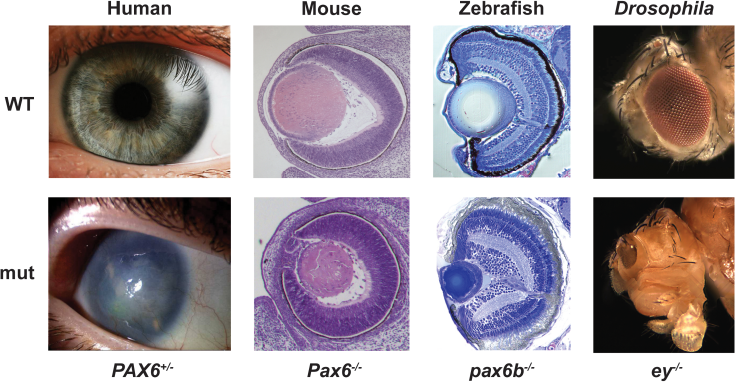
\includegraphics[width=0.5\textwidth]{fig03/PAX6_mutation.png}
  \caption{PAX6 alterations result in similar changes to eye morphology \newline (source: Washington et al, doi: 10.1371/journal.pbio.1000247 via \href{https://commons.wikimedia.org/w/index.php?curid=8626896}{Wikimedia Commons})}
\end{figure}

%
% Homologous and  analogous
%
\subsubsection*{Homologous and  analogous}
It is useful to check similarity at the molecular level because there are cases that analogous structures may not indicate homologous. 
\begin{figure}[H]
  \centering
      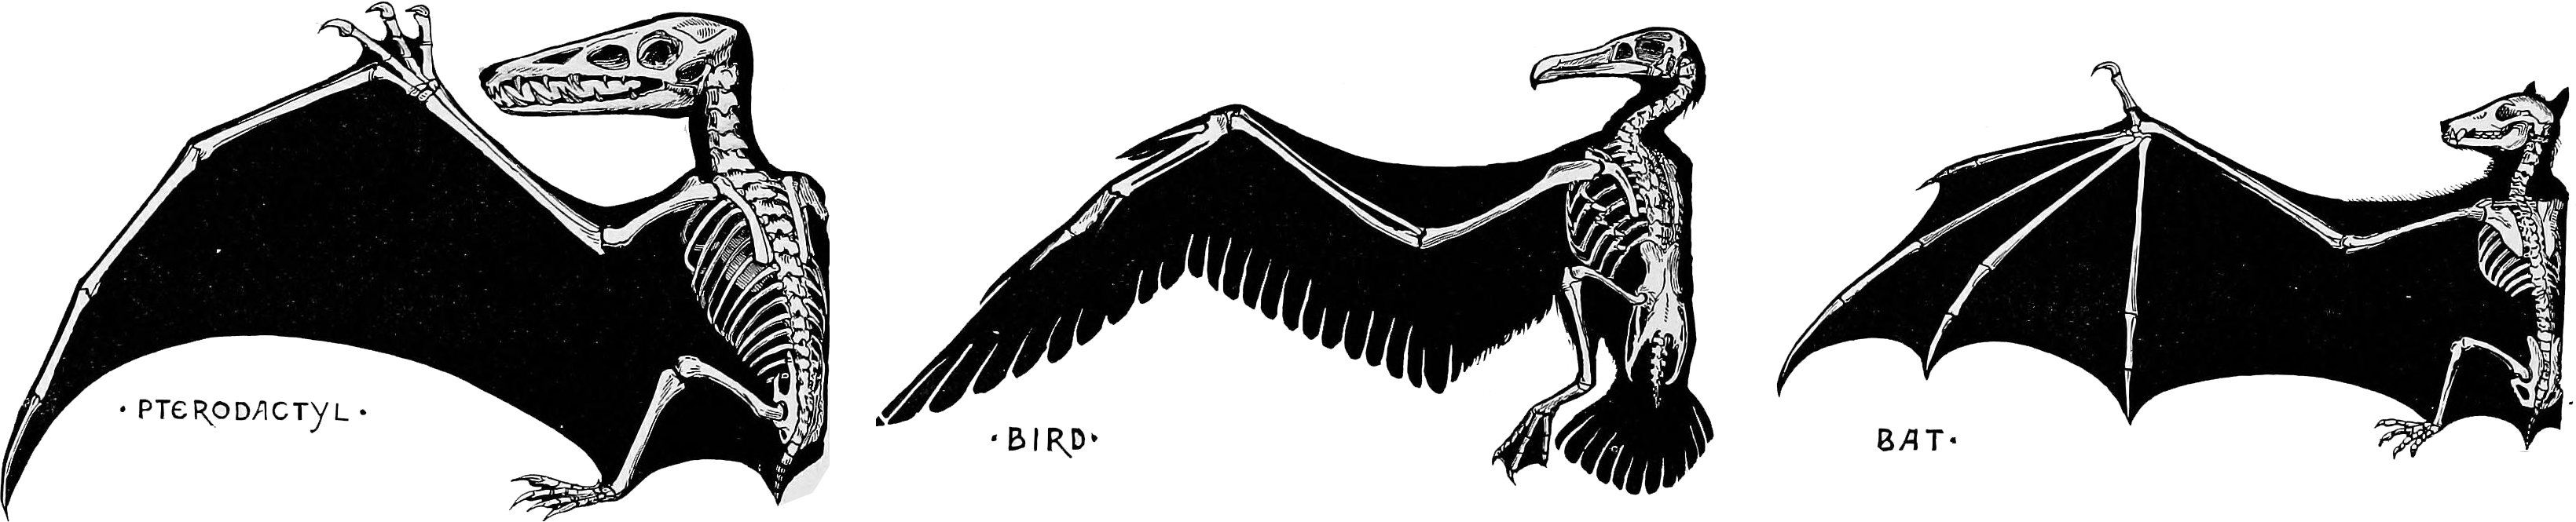
\includegraphics[width=0.5\textwidth]{fig03/analogous.png}
  \caption{Homologous and  analogous structures \newline (source: John Romanes, 1892, Darwin and after Darwin via \href{https://commons.wikimedia.org/w/index.php?curid=1324636}{Wikimedia Commons})}
\end{figure}

%
% Sequence homology
%
\subsubsection*{Sequence homology}
\begin{figure}[H]
  \centering
      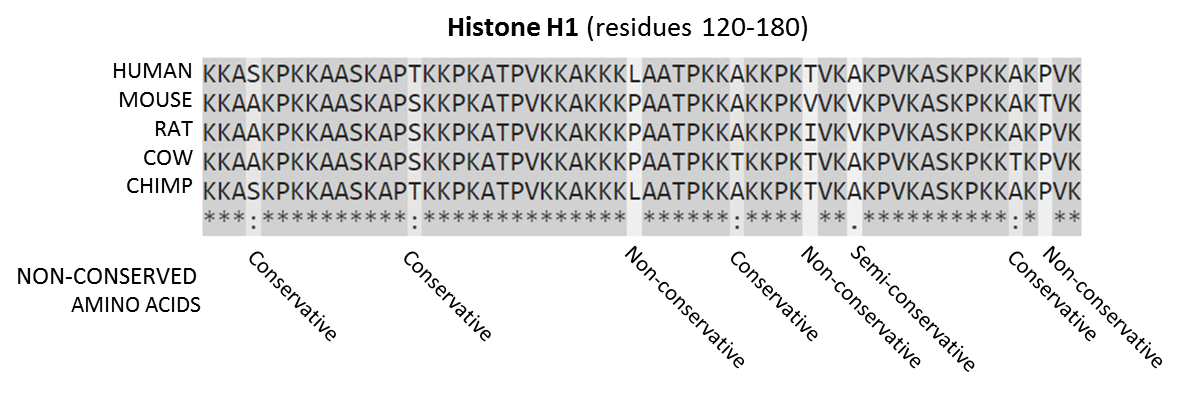
\includegraphics[width=0.75\textwidth]{fig03/histone_alignment.png}
  \caption{Multiple sequence alignment of histon sequences \newline (source: \href{https://commons.wikimedia.org/w/index.php?curid=37188728}{Shafee, Wikimedia Commons})}
\end{figure}

%
% Sequence homology
%
\subsubsection*{Evolution at the sequence level}
Sequence differences in DNA
\begin{itemize}
\item Substitution (a mismatch in alignment)
\item Insertion (a gap in alignment)
\item Deletion (a gap in alignment)
\item Inversion
\end{itemize}

\noindent
Source of variations
\begin{itemize}
\item Mutation
\item Recombination
\item Insertional mutagenesis
\item ...
\end{itemize}

\noindent
A mutation of the third nucleotide in a codon often does not affect which amino acid is synthesized.
\begin{itemize}
\item GCU $\rightarrow$ Ala (Alanine)
\item GCC $\rightarrow$ Ala (Alanine)
\item GCA $\rightarrow$ Ala (Alanine)
\item GCG $\rightarrow$ Ala (Alanine)
\end{itemize}

\noindent
An amino acid can be replaced by a different amino acid that has similar properties in some cases.
\begin{itemize}
\item AUU, AUC, AUA $\rightarrow$ Ile (Isoleucine)
\item CUU, CUC, CUA $\rightarrow$ Leu (Leucine)
\end{itemize}

%
% Extension of global alignment
%
\subsubsection*{Extension of global alignment with DP}

\begin{itemize}
\item Score matrix \\
DNA, RNA, and protein

\item Gap penatlty \\
Linear, affine, and constant
\end{itemize}



%\end{document}

\newpage
%\documentclass[12pt]{article}
%\usepackage[a4paper, margin=1in]{geometry} 
%\usepackage{graphicx} 
%\usepackage{hyperref}
%\usepackage{float}
%\usepackage{multicol}
%\usepackage[font=small, labelfont=bf]{caption}
%
%\begin{document}

%
% Introduction of score matrix
%
\subsection{Introduction of score matrix}
We will expand our simple scoring scheme to score matrices. This expansion allows us to solve general alignment problems with DNA, RNA, and protein sequences. 

%
% Extension of a scoring scheme to a score matrix
%
\subsubsection*{Extension of a scoring scheme to a score matrix}
The matrix below is equivalent with match: 1 and mismatch: 0. 

\begin{figure}[H]
  \centering
      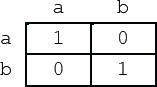
\includegraphics[width=0.175\textwidth]{fig03/simple_score_matrix.png}
\end{figure}

\noindent
\textbf{Example of a DNA score matrix}

\noindent
The matrix below is equivalent with match: 5 and mismatch: -4. 

\begin{figure}[H]
  \centering
      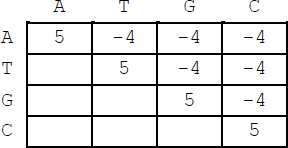
\includegraphics[width=0.3\textwidth]{fig03/dna_matrix_exercise.png}
\end{figure}

%
% Applications of score matrix
%
\subsubsection*{Applications of score matrix}

Score matrices are more flexible than the simple scoring scheme. For instance, they can be used for the following cases.

\begin{itemize}
\item DNA pairs
\item RNA pairs
\item Similarity of protein sequences by amino acid properties
\end{itemize}

%
% DNA pairs (Watson-Crick pairs)
%
\subsubsection*{DNA pairs (Watson-Crick pairs)}
A thymine pairs with an adenine, and a cytosine pairs with a guanine.

\begin{figure}[H]
  \centering
      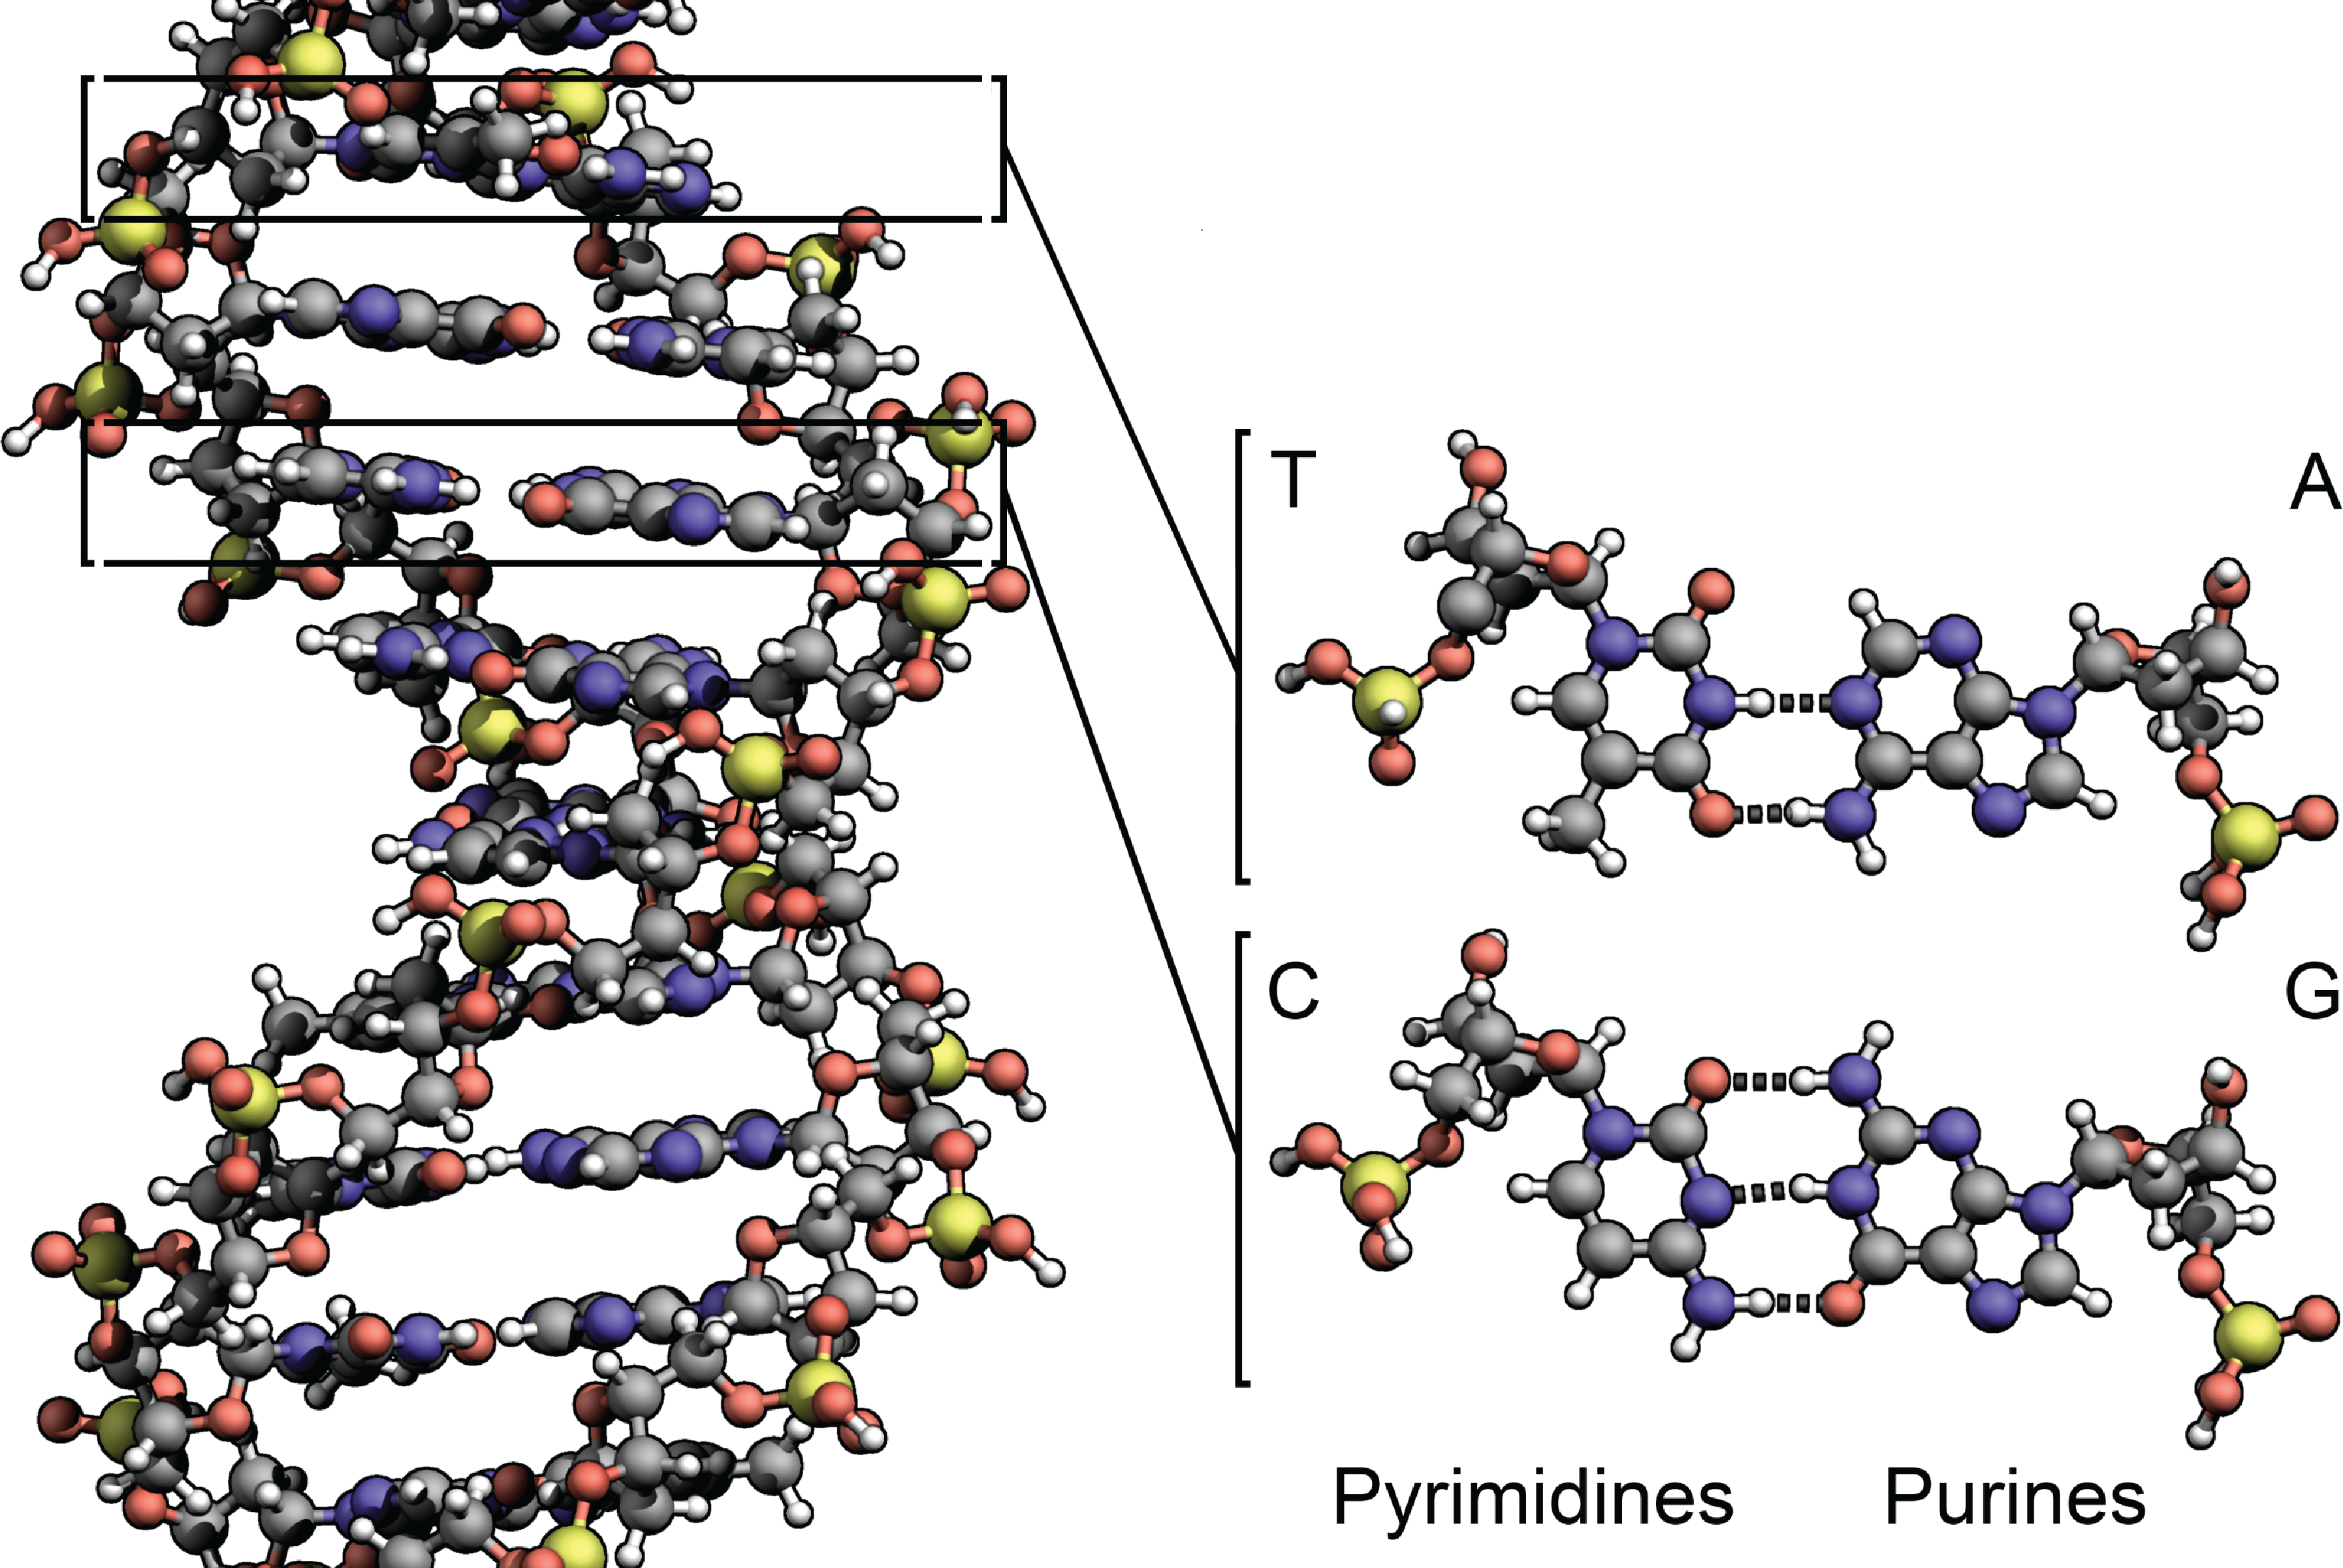
\includegraphics[width=0.4\textwidth]{fig03/dna_watson_crick_pair.png}
  \caption{Watson-Crick pairs (source: \href{https://commons.wikimedia.org/w/index.php?curid=15027555}{Zephyris, Wikimedia Commons})}
\end{figure}

%
% NEWPAGE
%
\newpage

\noindent \textbf{Example of score matrix for DNA pairs} \\
\noindent The matrix reflects the difference of hydrogen bonds.

\begin{figure}[H]
  \centering
      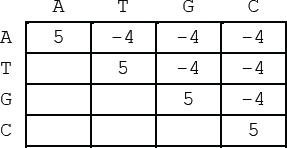
\includegraphics[width=0.3\textwidth]{fig03/example_dna_score_matrix.png}
\end{figure}

\noindent \textbf{Example of DP for DNA pairs} \\
\noindent You can use DP to find a DNA alignment with Watson-Crick pairs. For instance, the DP table below is used to solve the optimal alignment for two DNA sequences: q = AC and d = GT with gap penalty g = 4.

\begin{multicols}{2}
DP table:
\begin{figure}[H]
  \centering
      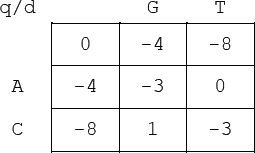
\includegraphics[width=0.25\textwidth]{fig03/example_watson_crick_alignment.png}
\end{figure}

Alignment:
\begin{verbatim}
    q: AC-
    d: -GT
\end{verbatim}

\end{multicols} 

%
% RNA pairs (Watson-Crick pairs)
%
\subsubsection*{RNA pairs}
A single stand of RNA can form a 3D structure that has a biological function. The secondary structure of RNA is a two-dimensional representation of the structure. 

\begin{figure}[H]
  \centering
      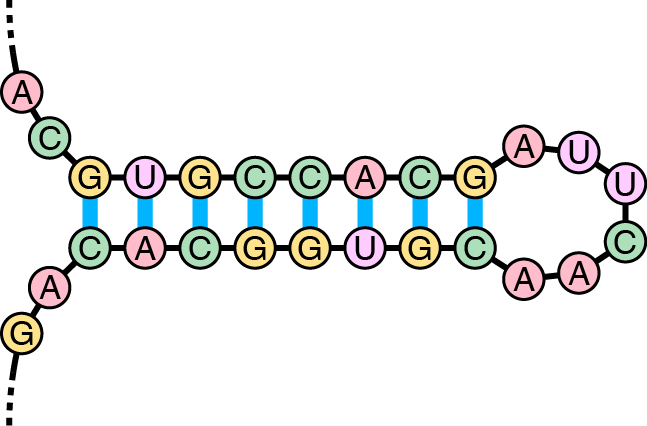
\includegraphics[width=0.3\textwidth]{fig03/rna_stem_loop.png}
  \caption{RNA stem-loop (source: \href{https://commons.wikimedia.org/w/index.php?curid=815268}{Sakurambo, Wikimedia Commons})}
\end{figure}

\noindent \textbf{Wobble pairs} \\
\noindent Wobble pairs are not canonical Watson-Crick pairs, but they can still form hydrogen bonds.

\begin{figure}[H]
  \centering
      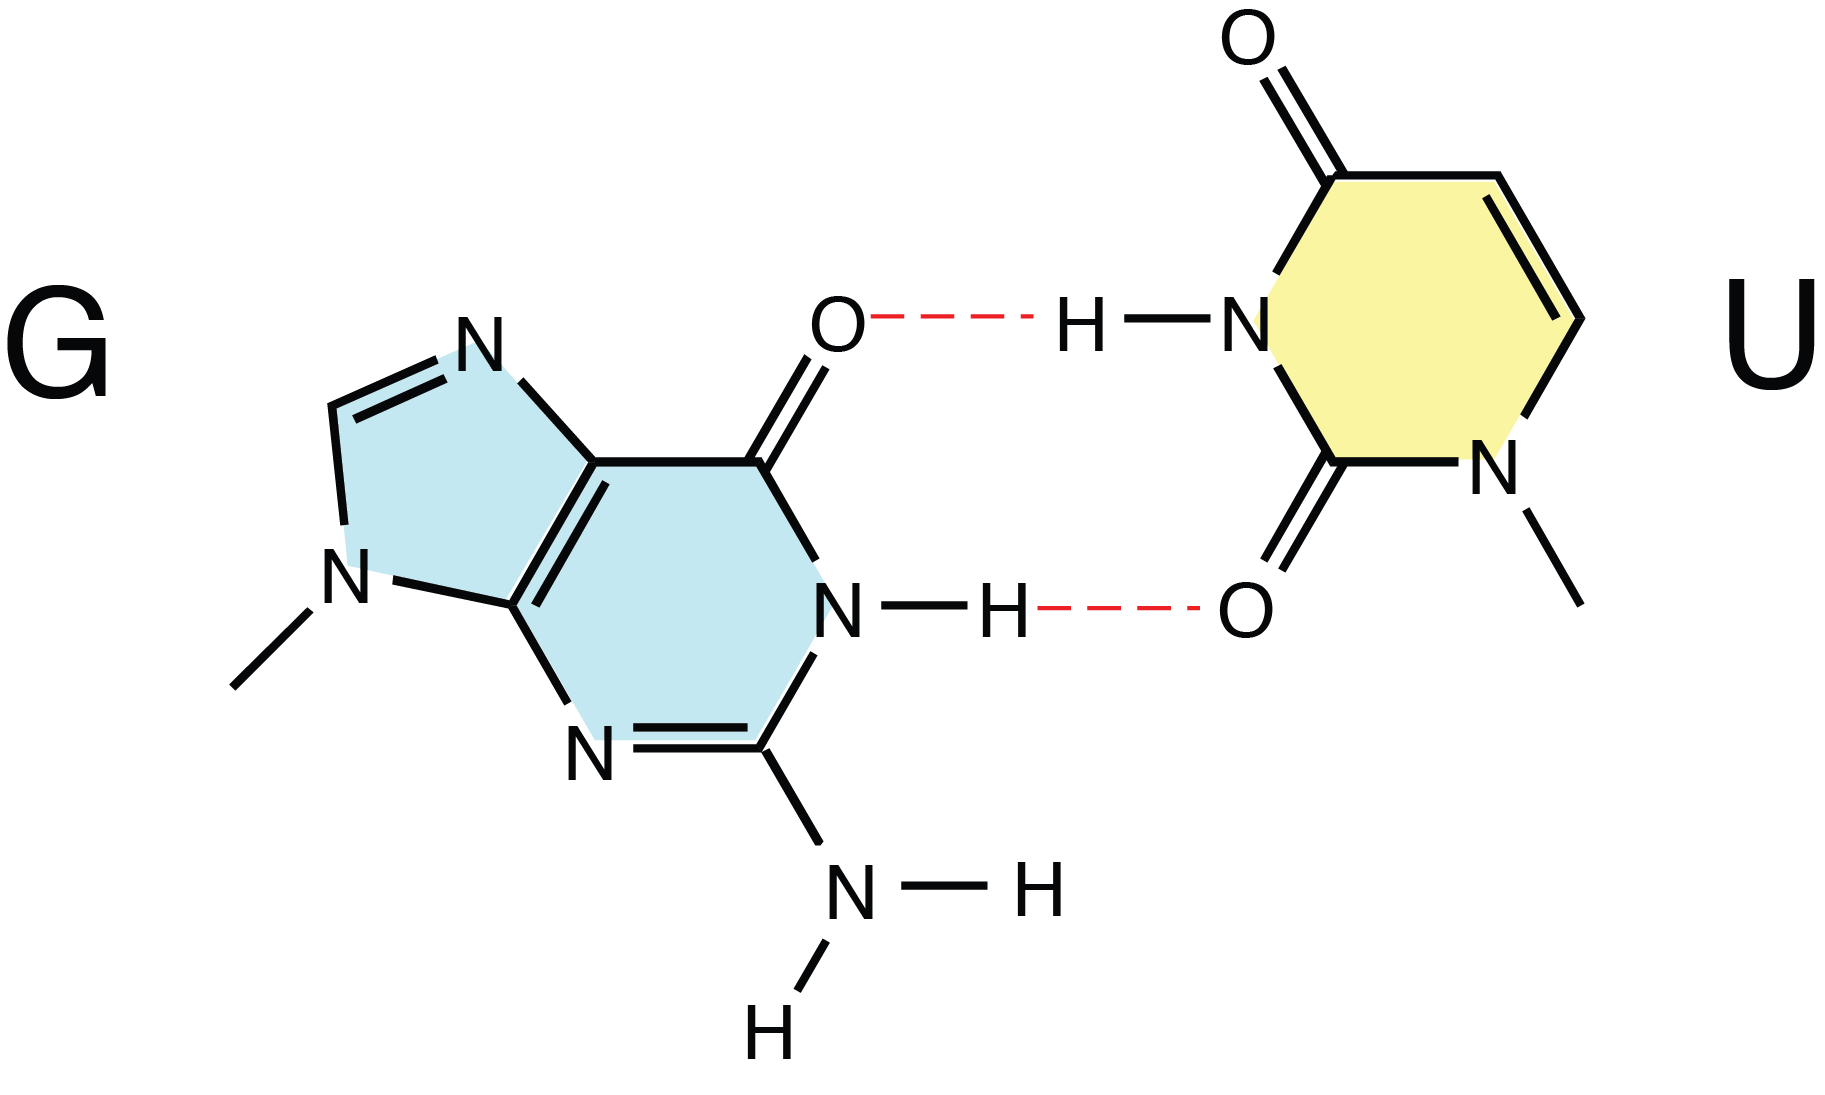
\includegraphics[width=0.3\textwidth]{fig03/rna_gu_wobble.png}
  \caption{GU wobble pairs \newline (modified  from the original version by \href{https://commons.wikimedia.org/w/index.php?curid=2636730}{Fdardel, Wikimedia Commons})}
\end{figure}

\noindent \textbf{Example of DP for RNA pairs} \\
\noindent You can form the following DP table for two RNA sequences: q = AU and d = UGA with gap penalty g = 9.
\begin{multicols}{2}
DP table:
\begin{figure}[H]
  \centering
      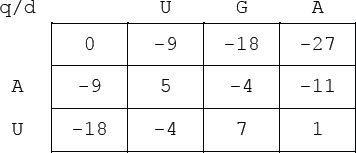
\includegraphics[width=0.25\textwidth]{fig03/example_rna_alignment.png}
\end{figure}

Alignment:
\begin{verbatim}
    q: A-U
    d: UGA
\end{verbatim}

\end{multicols} 

%
% Similarity of protein sequences
%
\subsubsection*{Similarity of protein sequences}
Amino acids can be categorized into several groups by their properties. Proteins alignments often need to take these properties into consideration.

\begin{figure}[H]
  \centering
      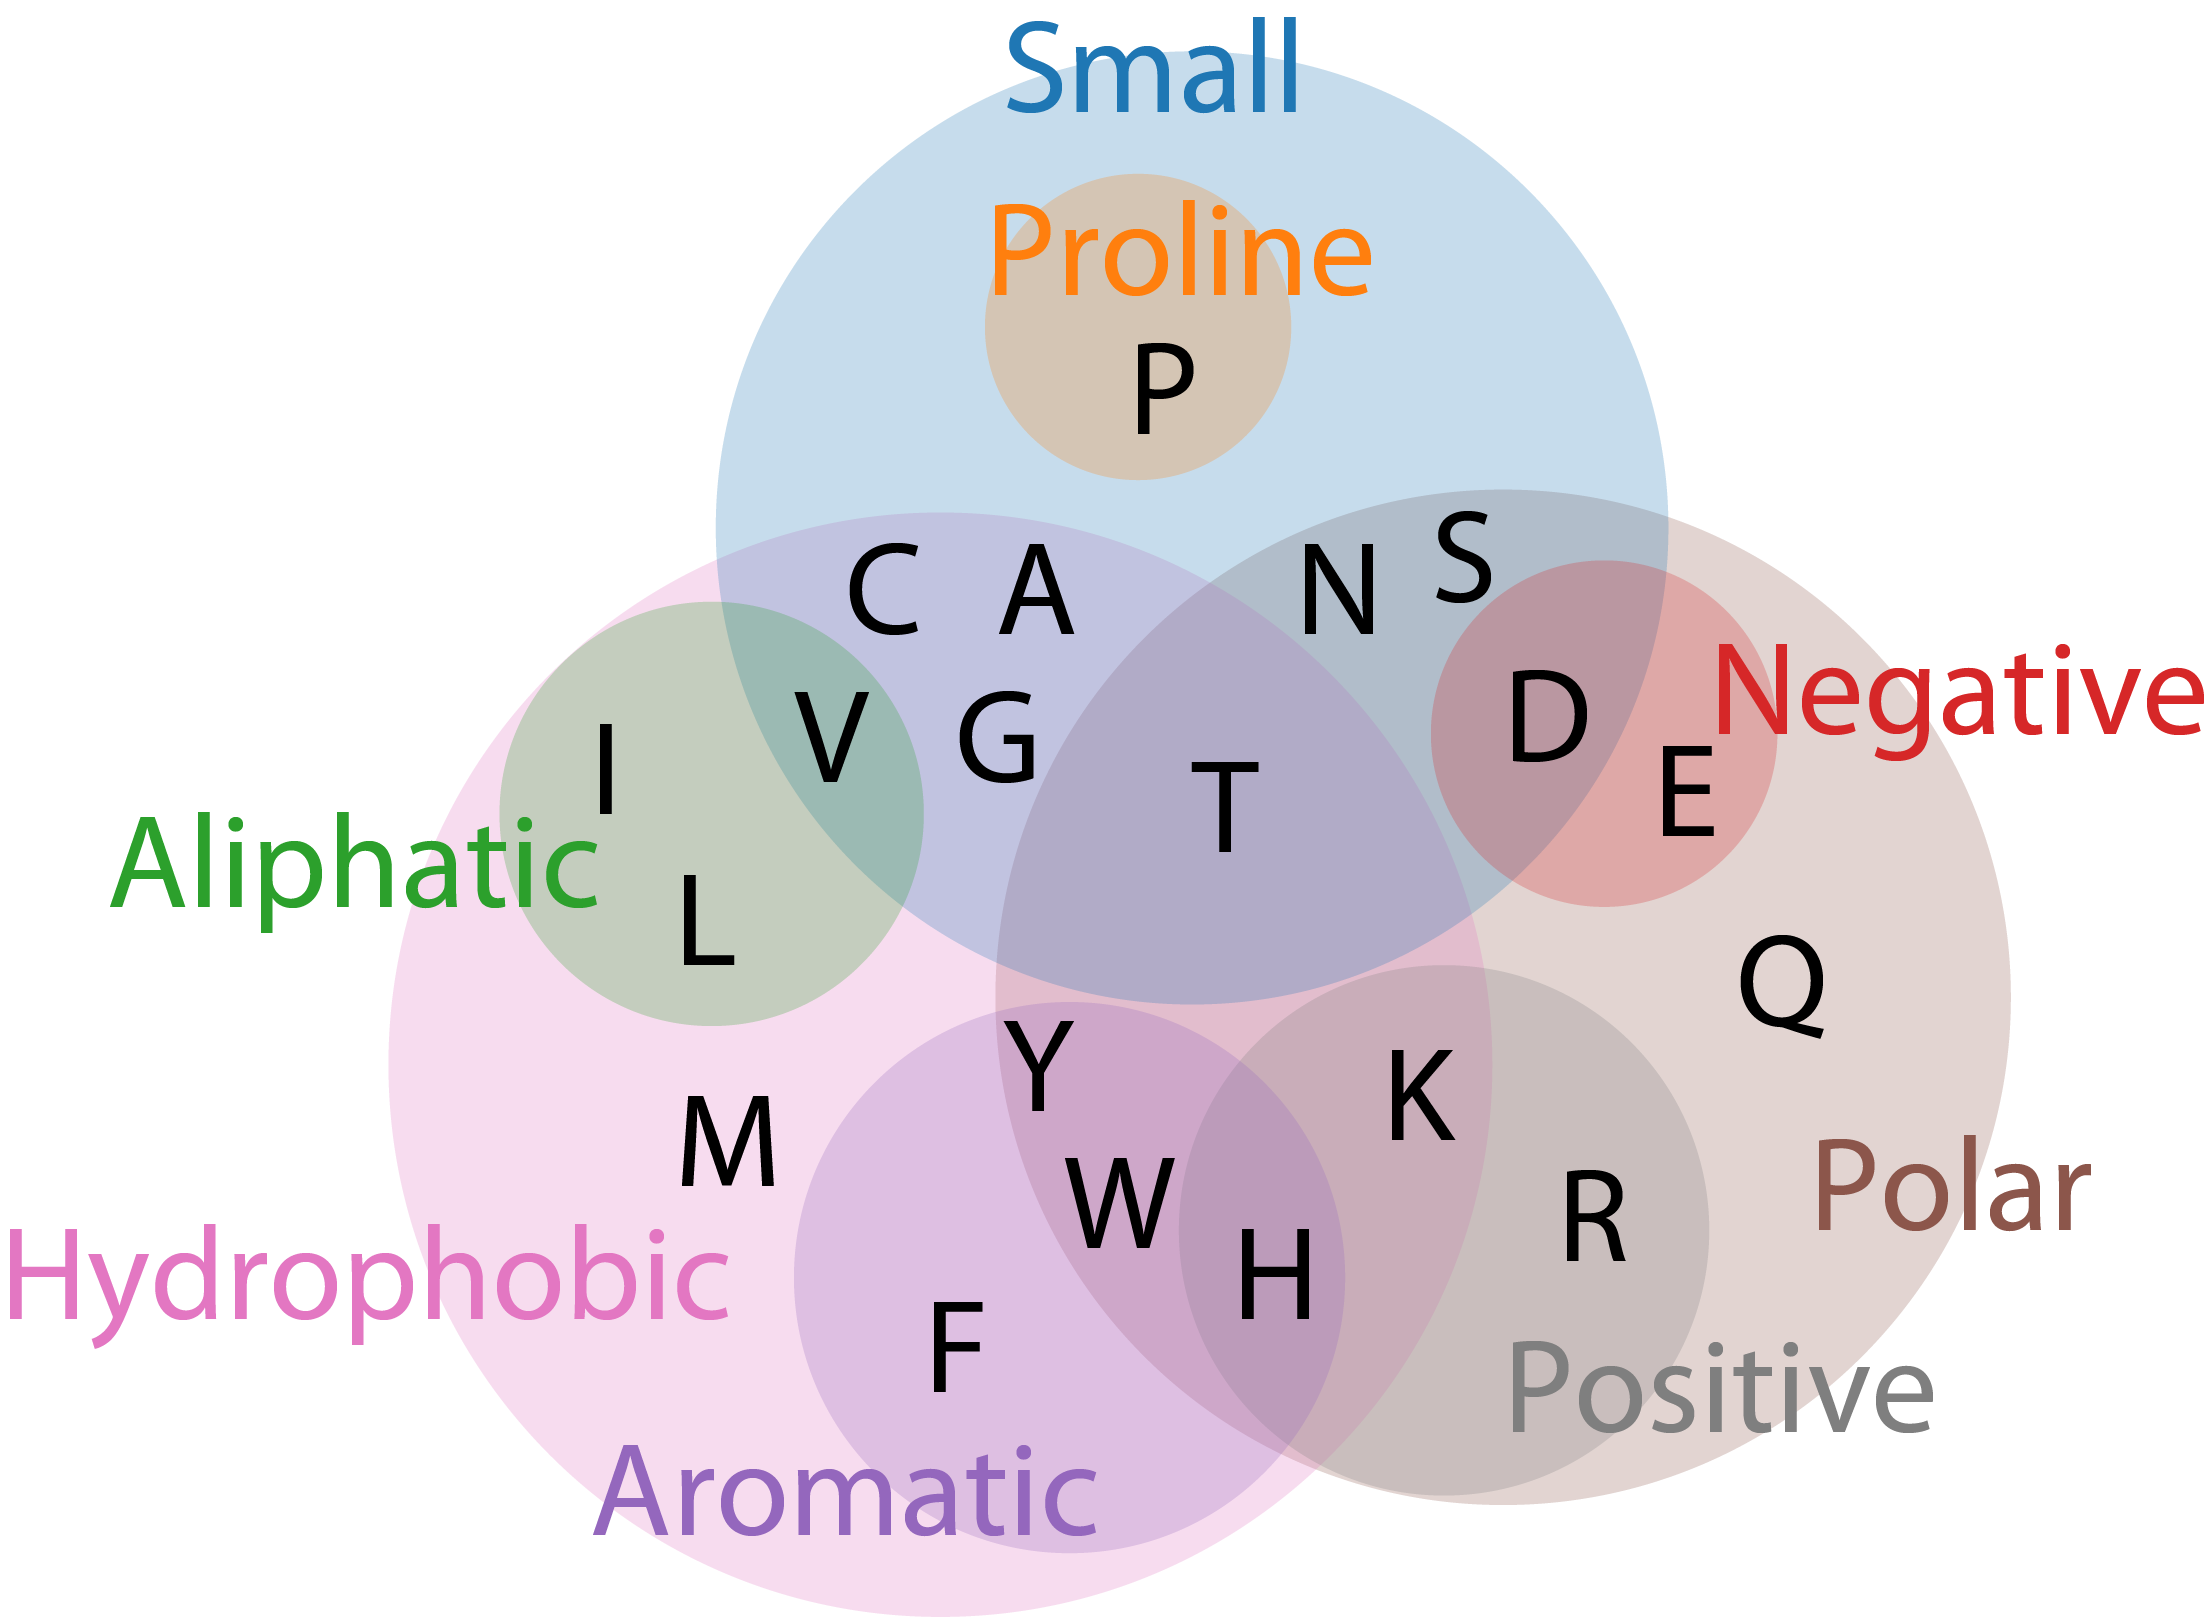
\includegraphics[width=0.3\textwidth]{fig03/amino_acid_properties.png}
  \caption{Venn diagram of amino acid properties }
\end{figure}

\noindent
\textbf{Example of a protein score matrix}\\
It can be used to compare the similarity between two protein sequences.

\begin{table}[!ht]
\footnotesize
\centering

\label{my-label}
\begin{tabular}{lllllllllllllllllllll}
   & \textbf{A }  & \textbf{R}   & \textbf{N}   & \textbf{D }  & \textbf{C}   & \textbf{Q}   & \textbf{E}   & \textbf{G}   & \textbf{H }  & \textbf{I}   & \textbf{L}   & \textbf{K}   & \textbf{M}   & \textbf{F}   & \textbf{P}   & \textbf{S}   & \textbf{T}   & \textbf{W}   & \textbf{Y}   & \textbf{V}   \\
\textbf{A} & 13  & 6   & 9   & 9   & 5   & 8   & 9   & 12  & 6   & 8   & 6   & 7   & 7   & 4   & 11  & 11  & 11  & 2   & 4   & 9   \\
\textbf{R} & 3   & 17  & 4   & 3   & 2   & 5   & 3   & 2   & 6   & 3   & 2   & 9   & 4   & 1   & 4   & 4   & 3   & 7   & 2   & 2   \\
\textbf{N} & 4   & 4   & 6   & 7   & 2   & 5   & 6   & 4   & 6   & 3   & 2   & 5   & 3   & 2   & 4   & 5   & 4   & 2   & 3   & 3   \\
\textbf{D} & 5   & 4   & 8   & 11  & 1   & 7   & 10  & 5   & 6   & 3   & 2   & 5   & 3   & 1   & 4   & 5   & 5   & 1   & 2   & 3   \\
\textbf{C} & 2   & 1   & 1   & 1   & 52  & 1   & 1   & 2   & 2   & 2   & 1   & 1   & 1   & 1   & 2   & 3   & 2   & 1   & 4   & 2   \\
\textbf{Q} & 3   & 5   & 5   & 6   & 1   & 10  & 7   & 3   & 7   & 2   & 3   & 5   & 3   & 1   & 4   & 3   & 3   & 1   & 2   & 3   \\
\textbf{E }& 5   & 4   & 7   & 11  & 1   & 9   & 12  & 5   & 6   & 3   & 2   & 5   & 3   & 1   & 4   & 5   & 5   & 1   & 2   & 3   \\
\textbf{G} & 12  & 5   & 10  & 10  & 4   & 7   & 9   & 27  & 5   & 5   & 4   & 6   & 5   & 3   & 8   & 11  & 9   & 2   & 3   & 7   \\
\textbf{H} & 2   & 5   & 5   & 4   & 2   & 7   & 4   & 2   & 15  & 2   & 2   & 3   & 2   & 2   & 3   & 3   & 2   & 2   & 3   & 2   \\
\textbf{I }& 3   & 2   & 2   & 2   & 2   & 2   & 2   & 2   & 2   & 10  & 6   & 2   & 6   & 5   & 2   & 3   & 4   & 1   & 3   & 9   \\
\textbf{L} & 6   & 4   & 4   & 3   & 2   & 6   & 4   & 3   & 5   & 15  & 34  & 4   & 20  & 13  & 5   & 4   & 6   & 6   & 7   & 13  \\
\textbf{K} & 6   & 18  & 10  & 8   & 2   & 10  & 8   & 5   & 8   & 5   & 4   & 24  & 9   & 2   & 6   & 8   & 8   & 4   & 3   & 5   \\
\textbf{M} & 1   & 1   & 1   & 1   & 0   & 1   & 1   & 1   & 1   & 2   & 3   & 2   & 6   & 2   & 1   & 1   & 1   & 1   & 1   & 2   \\
\textbf{F} & 2   & 1   & 2   & 1   & 1   & 1   & 1   & 1   & 3   & 5   & 6   & 1   & 4   & 32  & 1   & 2   & 2   & 4   & 20  & 3   \\
\textbf{P} & 7   & 5   & 5   & 4   & 3   & 5   & 4   & 5   & 5   & 3   & 3   & 4   & 3   & 2   & 20  & 6   & 5   & 1   & 2   & 4   \\
\textbf{S} & 9   & 6   & 8   & 7   & 7   & 6   & 7   & 9   & 6   & 5   & 4   & 7   & 5   & 3   & 9   & 10  & 9   & 4   & 4   & 6   \\
\textbf{T} & 8   & 5   & 6   & 6   & 4   & 5   & 5   & 6   & 4   & 6   & 4   & 6   & 5   & 3   & 6   & 8   & 11  & 2   & 3   & 6   \\
\textbf{W} & 0   & 2   & 0   & 0   & 0   & 0   & 0   & 0   & 1   & 0   & 1   & 0   & 0   & 1   & 0   & 1   & 0   & 55  & 1   & 0   \\
\textbf{Y} & 1   & 1   & 2   & 1   & 3   & 1   & 1   & 1   & 3   & 2   & 2   & 1   & 2   & 15  & 1   & 2   & 2   & 3   & 31  & 2   \\
\textbf{V} & 7   & 4   & 4   & 4   & 4   & 4   & 4   & 4   & 5   & 4   & 15  & 10  & 4   & 10  & 5   & 5   & 5   & 72  & 4   & 17 
\end{tabular}
\caption{Mutation probability matrix for the evolutionary distance of 250 PAMs (in percentage) (Chapter 22: A model of evolutionary change in proteins, Dayhoff and Schwartz, Atlas of Protein Sequence and Structure, 1978)}
\end{table}

%
% Exercise \thesection.1
%
\subsubsection*{Exercise \thesection.1}
\begin{enumerate}
\item Use the DNA score matrix below with g = 10 and find the optimal alignment for q = TG and d = TCG.

\begin{figure}[H]
  \centering
      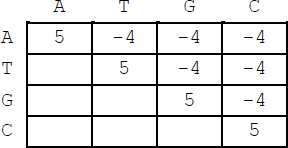
\includegraphics[width=0.25\textwidth]{fig03/dna_matrix_exercise.png}
\end{figure}

\item The 250 PAM mutation matrix above can not directly be used for global alignments. Explain what kind of matrix you need for calculating  alignment scores.
\end{enumerate}

\bigskip 

%\end{document}

%\documentclass[12pt]{article}
%\usepackage[a4paper, margin=1in]{geometry} 
%\usepackage{graphicx} 
%\usepackage{hyperref}
%\usepackage{float}
%\usepackage{multicol}
%\usepackage[font=small, labelfont=bf]{caption}
%
%\begin{document}

%
% Extension of gap penalties
%
\subsection{Extension of gap penalties}

%
% Types of gap penalties
%
\subsubsection*{Types of gap penalties}
Three types of gap penalties can be considered when creating an alignment. They treat a gap penalty differently depending on the gap length.

\begin{itemize}
\item Linear
\item Affine
\item Constant
\end{itemize}

%
% Gap penalty notation
%
\subsubsection*{Gap penalty notation}
\begin{itemize}
\item $g$: single gap penalty
\item $l$: length of a gap
\item $g_l$: gap penalty of length l
\item $g_{open}$: initial gap penalty
\item $g_{extend}$: extended gap penalty
\end{itemize}

%
% Linear gap penalty
%
\subsubsection*{Linear gap penalty}
It is the same as our simple scoring scheme. It treats a gap with multiple blanks as a result of several mutations. A gap of length $l$ can be calculated as: $g_l = g * l$.
\medskip 

\noindent
\textbf{Example of a gap of length 2}
\begin{verbatim}
    q: ACCCGT
    d: AC--GT
\end{verbatim}
The score of the gap (only the gap part) is 10 when $g$ = 5. 

%
% Affine gap penalty
%
\subsubsection*{Affine gap penalty}
It treats a gap with multiple blanks as a result of a single mutation. A gap with length $l$ can be calculated as: $g_l = g_{open} + (l – 1) * g_{extend}$.
\medskip 

\noindent
\textbf{Example of a gap of length 2}
\begin{verbatim}
    q: ACCCGT
    d: AC--GT
\end{verbatim}
The score of the gap (only the gap part) is 5.5 when $g_{open}$ and $g_{extend}$ are 5 and 0.5 respectively. 

%
% Constant gap penalty
%
\subsubsection*{Constant gap penalty}
It is similar to the affine gap penalty, but the score is independent form the gap length. A gap with length l can be calculated as: $g_l = g$ 
\medskip 

\noindent
\textbf{Example of a gap of length 2}
\begin{verbatim}
    q: ACCCGT
    d: AC--GT
\end{verbatim}
The score of the gap (only the gap part) for the alignment above is 5 when $g$ = 5. 

%
% Exercise \thesection.2
%
\subsubsection*{Exercise \thesection.2}
Calculate all three types of gap penalties for the gap in alignment 1 \& 2.

\begin{itemize}
\item $g$: 5
\item $g_{open}$: 5
\item $g_{extend}$: 0.5
\end{itemize}

\begin{multicols}{2}
\begin{verbatim}
Alignment 1
    q: CCCGG 
    d: CC-CG
\end{verbatim}

\begin{verbatim}
Alignment 2 
    q: CCCGG
    d: C---G
\end{verbatim}
\end{multicols}

%\end{document}


\end{document}


